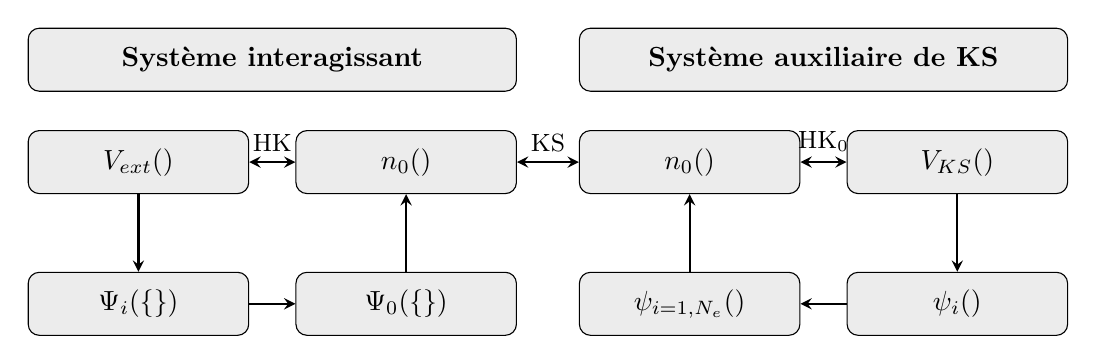
\begin{tikzpicture}[
    box/.style={rectangle, draw=black, rounded corners,
                fill=gray!15, minimum width=2.8cm,
                minimum height=0.8cm, align=center},
    arrow/.style={->, >=stealth, thick},
    darrow/.style={<->, >=stealth, thick}
]

% ---- Titres ----
\node[box, minimum width=6.2cm] at (-3.5, 2.5)
    {\textbf{Système interagissant}};
\node[box, minimum width=6.2cm] at (3.5, 2.5)
    {\textbf{Système auxiliaire de KS}};

% ---- Ligne du haut ----
\node[box] (vext)   at (-5.2,  1.2) {$V_\text{ext}(\rv)$};
\node[box] (n0l)    at (-1.8,  1.2) {$n_0(\rv)$};
\node[box] (n0r)    at ( 1.8,  1.2) {$n_0(\rv)$};
\node[box] (vks)    at ( 5.2,  1.2) {$V_\text{KS}(\rv)$};

% ---- Ligne du bas ----
\node[box] (psii)   at (-5.2, -0.6) {$\Psi_i(\{\rv\})$};
\node[box] (psi0)   at (-1.8, -0.6) {$\Psi_0(\{\rv\})$};
\node[box] (phiine) at ( 1.8, -0.6) {$\psi_{i=1,N_e}(\rv)$};
\node[box] (phii)   at ( 5.2, -0.6) {$\psi_i(\rv)$};

% ---- Flèches horizontales haut ----
\draw[darrow] (vext.east) -- (n0l.west)
    node[midway, above] {\small HK};
\draw[darrow] (n0l.east)  -- (n0r.west)
    node[midway, above] {\small KS};
\draw[darrow] (n0r.east)  -- (vks.west)
    node[midway, above] {\small HK$_0$};

% ---- Flèches verticales ----
\draw[arrow] (vext.south)   -- (psii.north);
\draw[arrow] (psi0.north)   -- (n0l.south);
\draw[arrow] (phiine.north) -- (n0r.south);
\draw[arrow] (vks.south)    -- (phii.north);

% ---- Flèches horizontales bas ----
\draw[arrow] (psii.east)  -- (psi0.west);
\draw[arrow] (phii.west)  -- (phiine.east);

\end{tikzpicture}